\documentclass{article}
\usepackage[paperwidth=5.8cm,paperheight=5.6cm,margin=3mm]{geometry}
\usepackage{amsmath}
\usepackage{tikz}
\usetikzlibrary{arrows.meta}
\pagestyle{empty}

\begin{document}
\begin{center}
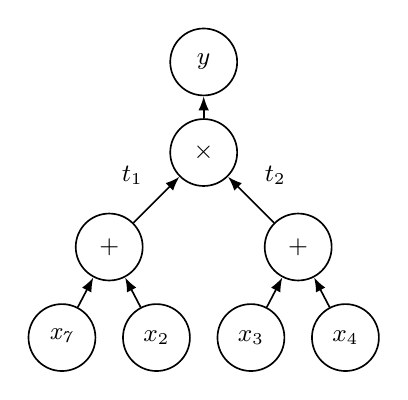
\begin{tikzpicture}[
  every node/.style={
    circle,
    draw,
    minimum size=8.5mm,
    inner sep=0pt,
    font=\small
  },
  every path/.style={
    -{Latex[length=1.8mm]},
    semithick
  }
]
	\node (x1) at (-1.8,0) {$\mathit{x_7}$};
  \node (x2) at (-0.6,0) {$x_2$};
  \node (x3) at (0.6,0) {$x_3$};
  \node (x4) at (1.8,0) {$x_4$};

  \node (add1) at (-1.2,1.15) {$+$};
  \node (add2) at (1.2,1.15) {$+$};

  \node (mul) at (0,2.35) {$\times$};
  \node (y) at (0,3.5) {$y$};

  \draw (x1) -- (add1);
  \draw (x2) -- (add1);
  \draw (x3) -- (add2);
  \draw (x4) -- (add2);
  \draw (add1) -- node[midway, above left, draw=none, circle=false, inner sep=1pt] {$t_1$} (mul);
  \draw (add2) -- node[midway, above right, draw=none, circle=false, inner sep=1pt] {$t_2$} (mul);
  \draw (mul) -- (y);
\end{tikzpicture}
\end{center}
\end{document}
